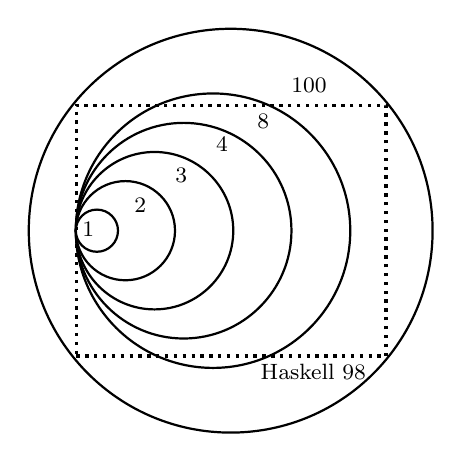
\begin{tikzpicture}[auto]
\footnotesize

\tikzstyle{variant}  = [draw, circle, thick, black, fill=white]
\tikzstyle{lbl}      = [black]

\draw [anchor=west]
  node [variant, text width=16.5em, xshift=-2em] (Var100) {}
  node [variant, text width=11em]  (Var8)   {}
  node [variant, text width=8.5em]  (Var4)   {}
  node [variant, text width=6em]  (Var3)   {}
  node [variant, text width=3.5em]  (Var2)   {}
  node [variant, text width=1em]  (Var1)   {}
  node [rectangle, draw, text width=12.5em, text height=10em, dotted, very thick, black] (HS98) {};

\node [lbl, above left of=Var100, xshift=5.7em, yshift=3.8em] {100};
\node [lbl, above left of=Var8, xshift=4.5em, yshift=2.3em] {8};
\node [lbl, above left of=Var4, xshift=4em, yshift=1.3em] {4};
\node [lbl, above left of=Var3, xshift=3.5em] {3};
\node [lbl, above left of=Var2, xshift=3em, yshift=-1.3em] {2};
\node [lbl, above left of=Var1, xshift=2em, yshift=-2.3em] {1};
\node [lbl, right, xshift=7.5em, yshift=-6em, very thick] (HS98.east) {Haskell 98};
\end{tikzpicture}
